\chapter{Introduction}

\gls{gui} are everywhere and are important for end users. \gls{gui}s connect users to software, and often are perceived as \emph{software}. \gls{gui}s often have input fields of various kinds, such as text boxes, checkboxes, drop-down lists, and so on. All of these different types of input fields oftentimes lead to complex dependencies between the fields. Consider an example of a graphical editing software, such as Adobe Illustrator\footnote{\url{https://www.adobe.com/no/products/illustrator.html}}. There, a user can manipulate the following values: absolute height, absolute width, relative height, relative width, each represented by a text box, and a Boolean indicator whether the ratio must be preserved. A change to any of these input fields must result in corresponding changes of other fields: indeed, for instance if the Boolean indicator is set to true, any changes to the width or height fields will be reflected to opposite field.

\gls{gui}s are often times wrong and buggy. 

In \autoref{fig:vaccine}, you can se a simple \gls{gui} form within a questioner. The error message is displayed, although the date on the from is within the specified boundaries.

\begin{figure}
    \centering
    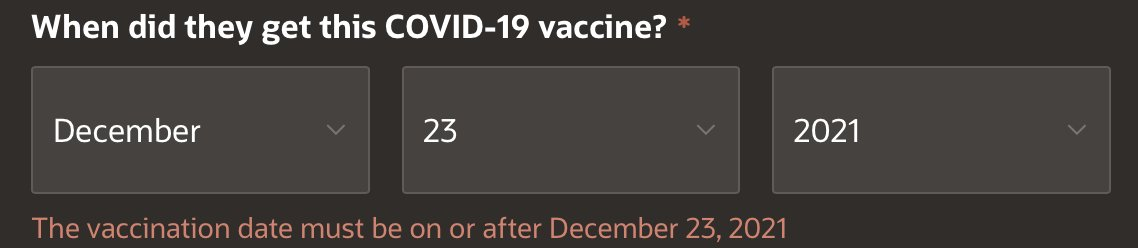
\includegraphics[scale=0.35]{figures/vaccine.jpeg}
    \caption{Example of a wrong validator}
    \label{fig:vaccine}
\end{figure}

The new system used by several universities in Norway, \gls{dfø}, has ambiguously formulated question throughout the application. These questions make the application difficult to use, and in certain circumstances, the user is unsure what to click on. One of these questions is presented in the \autoref{fig:DFO} --- however, it is unclear what will happen if either of the buttons is pressed.

\begin{figure}
    \centering
    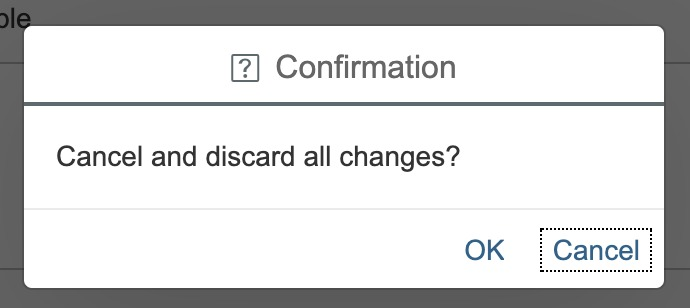
\includegraphics[scale=0.65]{figures/DFO.jpg}
    \caption{Example of an ambiguously formulated question}
    \label{fig:DFO}
\end{figure}

There are generally a lot of dependencies between all the fields in \gls{gui}s with forms that the user must fill out. As a result, they are more prone to make errors. One example of this is forms that has mandatory fields, this frequently leads to mistakes in field dependencies. In a form with several phases, you may be instructed to complete all required information before the form allows you to go back a step. This was the case in the registration form for \gls{pldi} conference --- shown in \autoref{fig:PLDI}. The user had to complete all required fields in the current phase before the \gls{gui} enabled the user to return to earlier phases. 
Another example of errors in forms is when the validation has a undesirable behavior. For instance, in a \gls{gui} with a form for writing down every travel abroad, such seen in \autoref{fig:enterfinland}. Due to incorrect validation, the user is unable to erase the first trip. Even though the details provided in the first trip, a validation error is shown, informing the user that the data is incorrect.
\begin{figure}
    \centering
    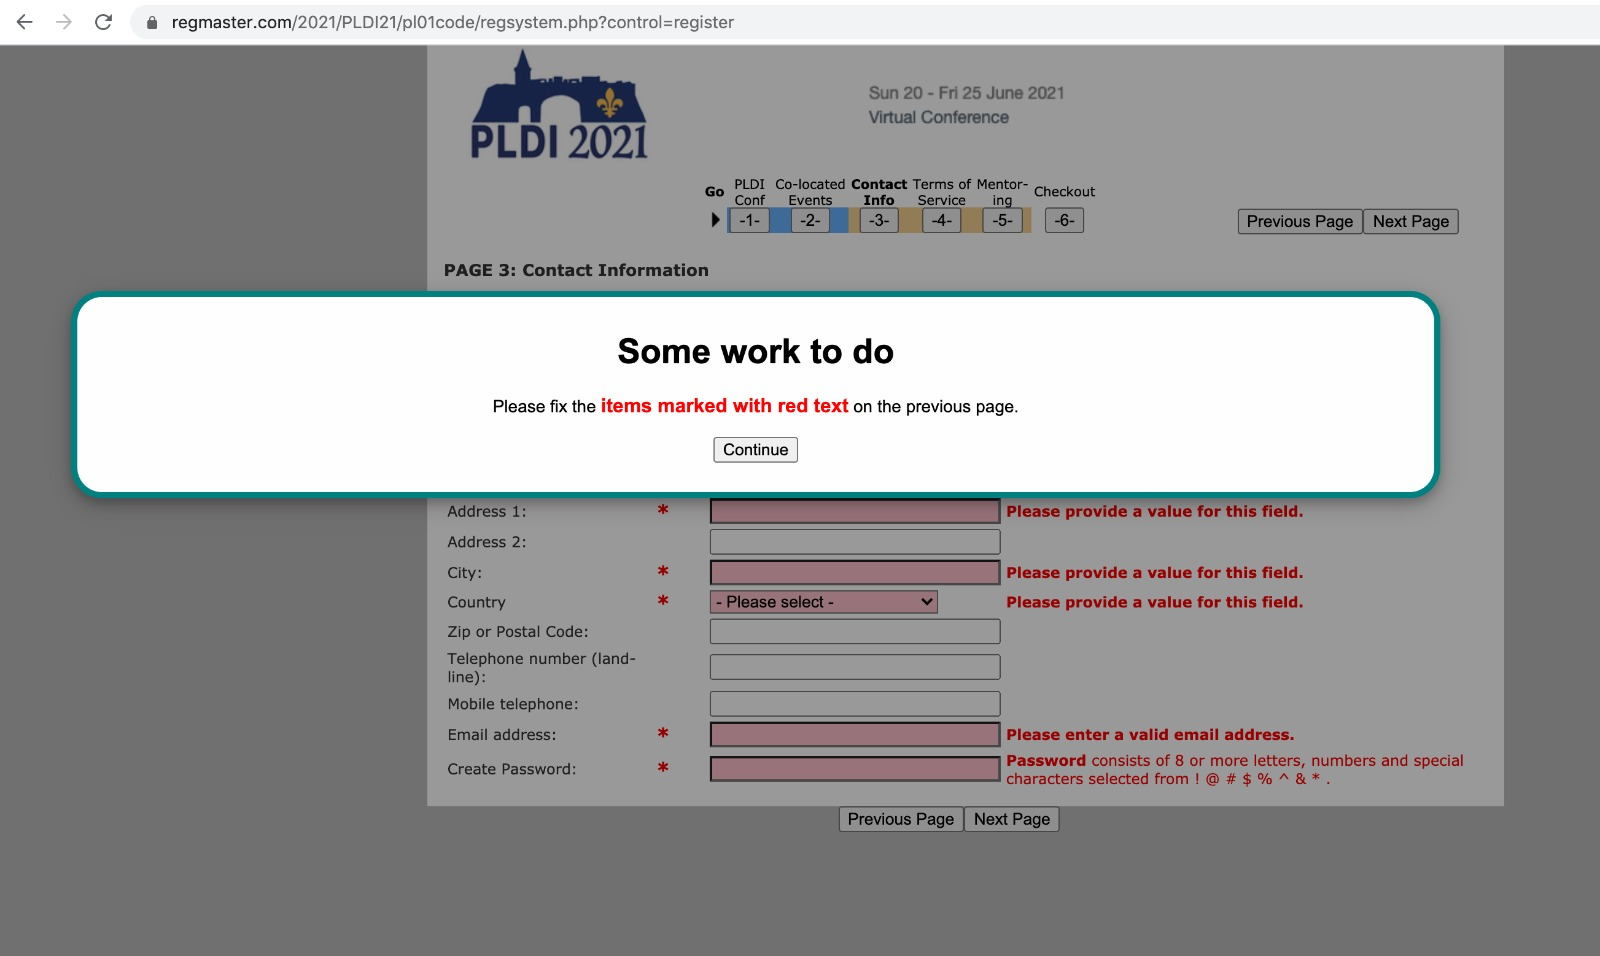
\includegraphics[scale=0.2]{figures/PLDI.jpg}
    \caption{Registration for a premier conference in programming languages}
    \label{fig:PLDI}
\end{figure}


\begin{figure}
    \caption{System for applying for Finnish citizenship}
    \centering
    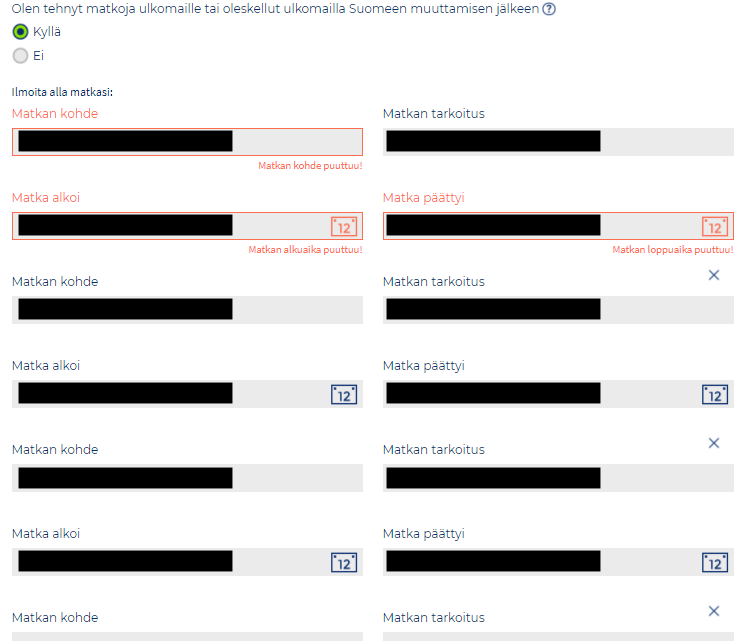
\includegraphics[scale=0.55]{figures/enterfinland-ui-citizenship-cant-remove-first-trip.png}
    \label{fig:enterfinland}
\end{figure}


\begin{figure}
    \centering
    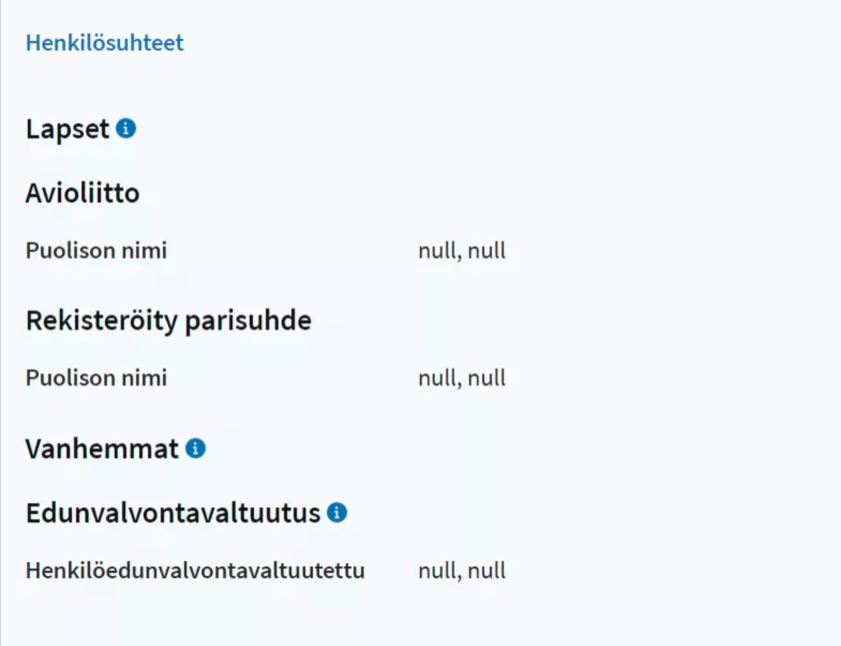
\includegraphics[scale=0.45]{figures/finnishSkatteetaten.png}
    \caption{Finnish tax system}
\end{figure}


This report is part of INF319 project at the \gls{uib}. The goal of the project was to understand event-based \gls{gui} programming and the limitation to such programming. Specify dataflow constraints and understand how they connect to \gls{gui} widgets. Understand the possibilities and limitations of constraint systems based on \gls{gui}s. The multiway dataflow constraint system used in the development of this project is HotDrink. Before developing this project I had no prior experience with the constraint system HotDrink. 
\\TODO: Skriv hva rapporten inneholder.
